\documentclass[tikz,border=6pt]{standalone}
\usepackage{pgfplots}
\pgfplotsset{compat=1.18}
\definecolor{rationalblue}{RGB}{37,99,235}
\definecolor{irrationalviolet}{RGB}{124,58,237}

\begin{document}
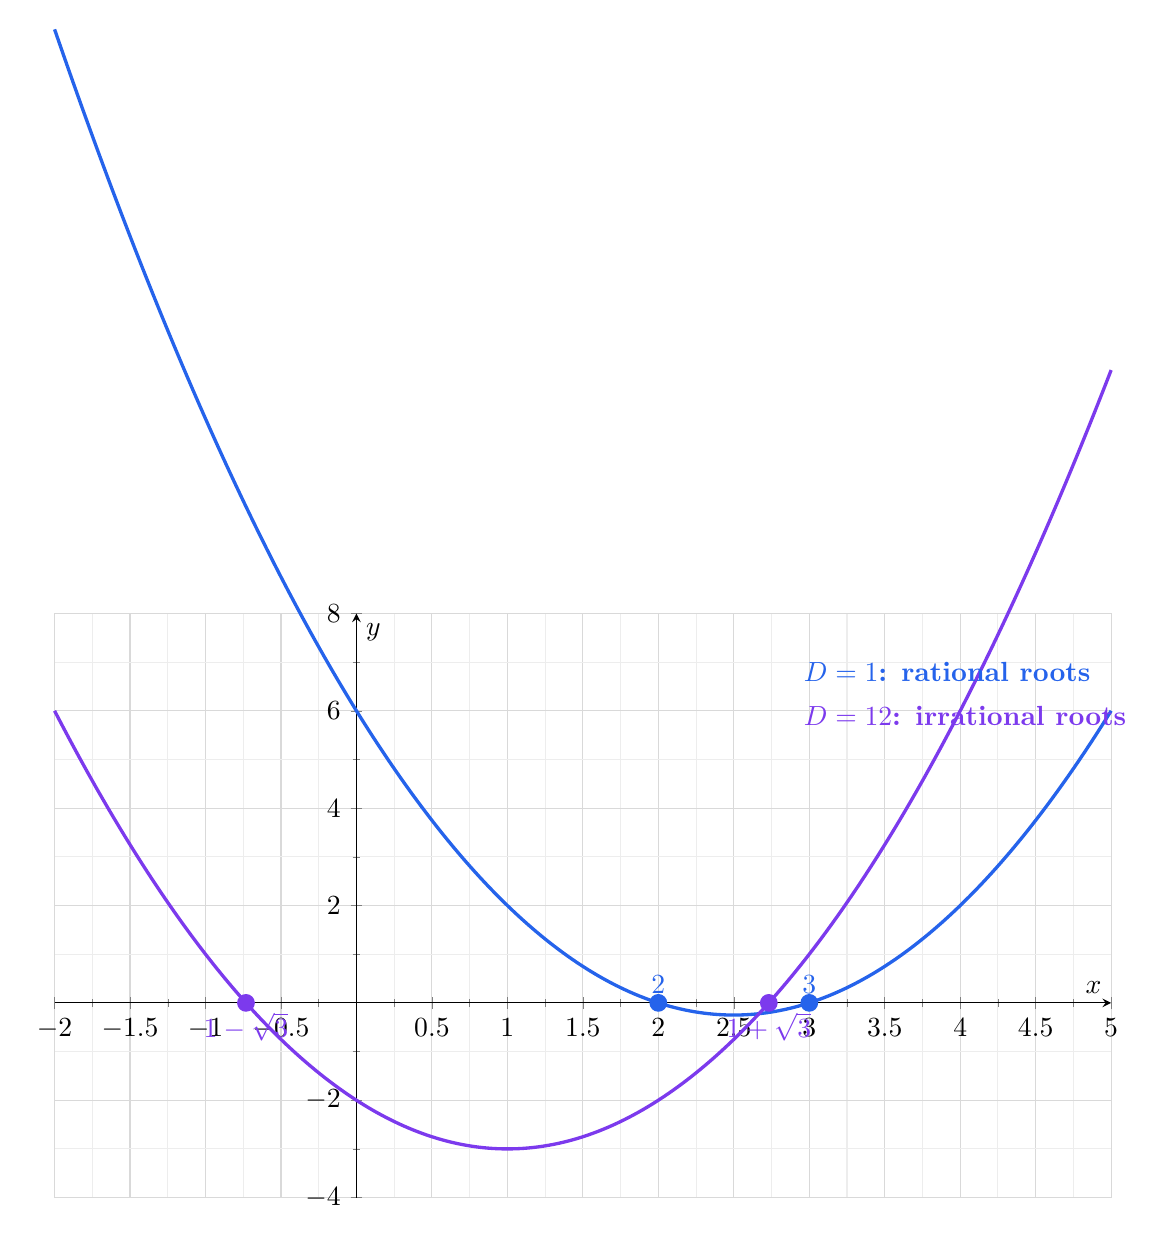
\begin{tikzpicture}
\begin{axis}[
  width=15cm,
  height=9cm,
  xmin=-2,
  xmax=5,
  ymin=-4,
  ymax=8,
  axis lines=middle,
  xlabel={$x$},
  ylabel={$y$},
  grid=both,
  minor tick num=1,
  major grid style={draw=gray!30},
  minor grid style={draw=gray!14},
  samples=240,
  clip=false
]

\addplot[rationalblue,very thick,domain=-2:5]{x^2-5*x+6};
\addplot[irrationalviolet,very thick,domain=-2:5]{x^2-2*x-2};

\addplot[rationalblue,only marks,mark=*,mark size=3pt]
  coordinates {(2,0) (3,0)};

\addplot[irrationalviolet,only marks,mark=*,mark size=3pt]
  coordinates {({1-sqrt(3)},0) ({1+sqrt(3)},0)};

\node[rationalblue,font=\bfseries,anchor=south]
  at (axis cs:2,0) {$2$};

\node[rationalblue,font=\bfseries,anchor=south]
  at (axis cs:3,0) {$3$};

\node[irrationalviolet,font=\bfseries,anchor=north]
  at (axis cs:{1-sqrt(3)},0) {$1-\sqrt3$};

\node[irrationalviolet,font=\bfseries,anchor=north]
  at (axis cs:{1+sqrt(3)},0) {$1+\sqrt3$};

\node[rationalblue,font=\bfseries,anchor=west]
  at (axis cs:2.9,6.8) {$D=1$: rational roots};

\node[irrationalviolet,font=\bfseries,anchor=west]
  at (axis cs:2.9,5.9) {$D=12$: irrational roots};

\end{axis}
\end{tikzpicture}
\end{document}
